%% ============================================================
%%  IEEE Conference Paper — IEEEtran class
%%  Title : Adaptive Physics-Constrained Loss Balancing in
%%          KAN-Enhanced Graph Neural Networks for Flood Forecasting
%%  Target: NeurIPS ClimateAI Workshop 2026 /
%%          AGU Annual Meeting 2026
%% ============================================================

\documentclass[conference]{IEEEtran}

%% ── Packages ─────────────────────────────────────────────────
\usepackage{cite}
\usepackage{amsmath,amssymb,amsfonts}
\usepackage{graphicx}
\usepackage{textcomp}
\usepackage{xcolor}
\usepackage{booktabs}
\usepackage{multirow}
\usepackage{url}
\usepackage{algorithm}
\usepackage{algorithmic}
\usepackage[hidelinks]{hyperref}
\usepackage{subcaption}
\usepackage{array}
\usepackage{tabularx}

%% ── Convenience math operators ───────────────────────────────
\DeclareMathOperator{\ReLU}{ReLU}
\newcommand{\norm}[1]{\left\lVert#1\right\rVert}

%% ── Prevent overfull hboxes in tight columns ─────────────────
\emergencystretch=2em

%% ── Figure path ──────────────────────────────────────────────
\graphicspath{{results/figures/}}

%% =============================================================
\begin{document}

\title{Adaptive Physics-Constrained Loss Balancing in\\
KAN-Enhanced Graph Neural Networks for Flood Forecasting}

\author{
  \IEEEauthorblockN{Sandeepan Ghosh}
  \IEEEauthorblockA{
    \textit{Department of Data Science and Business Systems}\\
    \textit{SRM Institute of Science and Technology}\\
    Chennai, India\\
    ss9737@srmist.edu.in
  }
  \and
  \IEEEauthorblockN{Vadivu G}
  \IEEEauthorblockA{
    \textit{Department of Data Science and Business Systems}\\
    \textit{SRM Institute of Science and Technology}\\
    Chennai, India\\
    vadivug@srmist.edu.in
  }
}

\maketitle

%% =============================================================
\begin{abstract}
Physics-informed graph neural networks (PIGNNs) have emerged as
computationally efficient surrogate models for large-scale flood
forecasting. The recently introduced HydroGraphNet framework
\cite{taghizadeh2025} demonstrates significant advances by integrating
Kolmogorov--Arnold Networks (KANs) within an encoder--processor--decoder
graph neural network architecture, achieving a 67\% reduction in
prediction error over baseline GNN methods on the White River, Muncie,
Indiana benchmark dataset. However, its physics-informed loss employs a
static weighting coefficient $\lambda_{phy}=1.0$, which is known to cause
gradient imbalance in PINN literature. In this work, we empirically
characterise this imbalance through three loss-weighting strategies: (1)
the fixed-weight baseline, (2) a linear warm-up schedule, and (3) gradient
norm balancing (GNB). Contrary to the canonical PINN assumption of physics
gradient dominance, our gradient norm measurements reveal that the physics
gradient is consistently 8--20$\times$ \emph{weaker} than the MSE gradient
($\rho \approx 0.04$--$0.13$) throughout training, caused by area
normalisation in the continuity loss formulation. The GNB strategy
automatically discovers this imbalance and amplifies $\lambda_{phy}$ to
5.0, yielding a \textbf{5.8\% reduction in RMSE} (0.02031 vs.\ 0.02157)
over the fixed baseline. The linear warm-up strategy achieves
$R^{2}=0.200$, a \textbf{25.8\% improvement} over the fixed baseline
($R^{2}=0.159$). Our work provides an implementable contribution on an open
benchmark and a corrected methodological framework for physics-informed GNN
training dynamics in hydrology.
\end{abstract}

\begin{IEEEkeywords}
Physics-Informed GNN, Flood Forecasting, Kolmogorov--Arnold Networks,
Adaptive Loss Balancing, Shallow Water Equations, Surrogate Modelling,
Gradient Norm Balancing
\end{IEEEkeywords}

%% =============================================================
\section{Introduction}
\label{sec:intro}

Floods are among the most destructive natural hazards globally, causing
over USD~651 billion in losses between 2000 and 2019 \cite{undrr2020}.
Traditional physics-based hydrodynamic models (e.g., HEC-RAS~2D) provide
high-fidelity simulations but require hours per flood event, making
real-time forecasting infeasible. Deep learning surrogate models trained on
simulation data offer orders-of-magnitude speedups; among these, graph
neural networks (GNNs) are particularly attractive because their
message-passing mechanism mirrors flood propagation over unstructured
spatial meshes.

HydroGraphNet \cite{taghizadeh2025}, implemented within NVIDIA
PhysicsNeMo, marks a significant step by combining: (i)~a $k$-nearest
neighbour GNN, (ii)~a physics-informed continuity loss enforced via ReLU
inequality constraints, and (iii)~KAN layers \cite{liu2024kan} in the node
encoder. Despite its strong benchmark results, its training objective:
\begin{equation}
  \mathcal{L}_{\text{total}} = \mathcal{L}_{\text{MSE}} +
  \lambda_{phy} \cdot \mathcal{L}_{\text{physics}}, \quad
  \lambda_{phy} = 1.0 \text{ (constant)}
  \label{eq:loss_static}
\end{equation}
uses a fixed weight throughout training. In broader PINN literature
\cite{wang2021}, this static approach is known to cause gradient conflict.

This paper makes four contributions:
\begin{enumerate}
  \item Formal characterisation of the physics loss and its area-normalised
        gradient suppression mechanism.
  \item Empirical gradient norm analysis revealing $\rho \ll 1$ (physics
        gradient is weak, not dominant) — contrary to prior PINN
        assumptions.
  \item An adaptive physics-constrained loss scheduling framework with
        three strategies, validated on the White River benchmark.
  \item Analysis of KAN placement and theoretical extensions toward local
        conservation and uncertainty quantification.
\end{enumerate}

%% =============================================================
\section{Related Work}
\label{sec:related}

\subsection{GNNs for Flood Modelling}
FloodGNN-GRU \cite{bentivoglio2023} combined spatial GNNs with GRU units
for spatio-temporal flood prediction but lacked physics constraints.
mSWE-GNN \cite{lino2025} introduced multi-scale graph pooling for
multi-resolution dynamics. DUALFloodGNN \cite{acosta2025} enforced local
and global mass conservation with curriculum learning, directly motivating
the present work.

\subsection{Physics-Informed Neural Networks in Hydrology}
Raissi et al.\ \cite{raissi2019} introduced PINNs by embedding PDE
residuals into the loss function. De la Fuente et al.\ \cite{delaFuente2023}
applied PINNs to 2D shallow water equations without labelled data; Haris et
al.\ \cite{haris2025} demonstrated that the physics-to-data loss ratio
requires careful calibration for river stage surrogate models.

\subsection{Kolmogorov--Arnold Networks}
Liu et al.\ \cite{liu2024kan} introduced KANs as interpretable
alternatives to MLPs using learnable spline functions on edges. FloodKAN
\cite{zhao2025} applied KANs to flood susceptibility mapping. HydroGraphNet
was the first to integrate KAN within a GNN for flood dynamics modelling.

\subsection{Adaptive Loss Weighting in PINNs}
Wang et al.\ \cite{wang2021} showed that unbalanced gradient magnitudes
disable one loss component in PINN training. Self-adaptive PINNs
\cite{mcclenny2023} use per-point weights; gradient surgery \cite{yu2020}
projects conflicting gradients. No prior work has applied adaptive loss
balancing specifically to physics-informed GNNs for flood forecasting.

%% =============================================================
\section{HydroGraphNet Architecture}
\label{sec:arch}

\subsection{Problem Formulation}
Let $\mathcal{G}=(\mathcal{V},\mathcal{E})$ be a spatial graph where node
$v_i\in\mathcal{V}$ corresponds to a computational cell, and $N=4{,}787$
nodes cover the White River basin. At each time step $t$ the model predicts
one-step residuals:
\begin{equation}
  \Delta h_i^{t+1} = h_i^{t+1} - h_i^t, \quad
  \Delta V_i^{t+1} = V_i^{t+1} - V_i^t
\end{equation}
accumulated autoregressively for multi-step rollout.

\subsection{Graph Construction}
Edges connect $k=4$ nearest neighbours by Euclidean distance; 3-D edge
features encode direction cosines and distance:
\begin{equation}
  \mathbf{e}_{ij} = \left[
    \tfrac{x_i-x_j}{\|\mathbf{x}_i-\mathbf{x}_j\|},\;
    \tfrac{y_i-y_j}{\|\mathbf{x}_i-\mathbf{x}_j\|},\;
    \|\mathbf{x}_i-\mathbf{x}_j\|
  \right] \in \mathbb{R}^3
\end{equation}

\subsection{Node Features}
Each node carries a 16-D feature vector:
\begin{align}
  \mathbf{x}_i &=
    \underbrace{[x_i,\,y_i,\,A_i,\,z_i,\,s_i,\,\alpha_i,\,
      \kappa_i,\,n_i,\,f_{\text{acc},i},\,\phi_i]}_{\text{static (10D)}}
    \nonumber\\
  &\quad\oplus\,
    \underbrace{[Q_{\text{in}}^t,\,P^t]}_{\text{global (2D)}}
    \oplus\,
    \underbrace{[h_i^{t-1},\,h_i^t]}_{\text{depth (2D)}}
    \oplus\,
    \underbrace{[V_i^{t-1},\,V_i^t]}_{\text{volume (2D)}}
\end{align}
All features are $z$-score normalised prior to input.

\subsection{MeshGraphKAN: Encoder--Processor--Decoder}
\textbf{Node encoder (KAN-based):}
\begin{equation}
  \mathbf{h}_i^{(0)} = \text{KAN}(\mathbf{x}_i;\,\theta_{enc})
  \in \mathbb{R}^{128}
\end{equation}
using $K=5$ Fourier harmonics per learnable edge function:
\begin{equation}
  \phi_q(x) = \sum_{k=1}^{K}\left[a_k\cos(k\pi x)+b_k\sin(k\pi x)\right]
\end{equation}

\noindent\textbf{Processor (15 message-passing layers):}
\begin{align}
  \mathbf{m}_{ij}^{(l)} &= \mathbf{m}_{ij}^{(l-1)}
    + \text{MLP}_{e}^{(l)}\!\left([\mathbf{h}_i^{(l-1)}\|
      \mathbf{h}_j^{(l-1)}\|\mathbf{m}_{ij}^{(l-1)}]\right) \\
  \mathbf{h}_i^{(l)} &= \mathbf{h}_i^{(l-1)}
    + \text{MLP}_{n}^{(l)}\!\left(
      \Bigl[\mathbf{h}_i^{(l-1)}\Big\|
      \sum_{j\in\mathcal{N}(i)}\mathbf{m}_{ij}^{(l)}\Bigr]\right)
\end{align}

\noindent\textbf{Node decoder (MLP-based):}
\begin{equation}
  \hat{\mathbf{y}}_i = \text{MLP}_{dec}\!\left(\mathbf{h}_i^{(15)}\right)
  \in \mathbb{R}^2
  \quad\text{encoding }(\Delta\hat{h}_i,\,\Delta\hat{V}_i)
\end{equation}
Total trainable parameters: 2,318,722.

%% =============================================================
\section{Physics-Informed Loss: Formulation and Limitations}
\label{sec:loss}

\subsection{Shallow Water Continuity Equation}
The integral continuity equation at node $i$ over $\Delta t = 1200$~s:
\begin{equation}
  V_i^{t+1} = V_i^t + \Delta t\cdot\left(Q_{\text{in}}^t
    + P^t\cdot A_{\text{inf}} - Q_{\text{out}}^t\right)
\end{equation}

\subsection{Global Continuity Loss}
HydroGraphNet enforces conservation at the domain level. Two ReLU
inequality constraints penalise violations:
\begin{align}
  \mathcal{L}_1 &= \left[\ReLU\!\left(
    \frac{\hat{V}_{\text{total}}^{t+1}
      - \bigl(\bar{V}^t_{d} + \Delta t({\bar{Q}}_{\text{in}}^t
        + \bar{P}^t A_{\text{inf}})\bigr)}
      {A_{\text{sum}}}\right)\right]^2 \\
  \mathcal{L}_2 &= \left[\ReLU\!\left(
    \frac{V^{t+1}_{d} - \hat{V}_{\text{total}}^{t+1}
      - \Delta t(Q_{\text{in}}^{t+1}+P^{t+1}A_{\text{inf}})}
      {A_{\text{sum}}}\right)\right]^2 \\
  \mathcal{L}_{\text{physics}} &=
    \frac{1}{B}\sum_{b=1}^{B}\bigl(\mathcal{L}_1^b+\mathcal{L}_2^b\bigr)
\end{align}
where $A_{\text{sum}}$ is the total domain area.

\subsection{Identified Limitations}

\textbf{L1 — Gradient Suppression via Area Normalisation.}
Both constraints are divided by $A_{\text{sum}}$, reducing the physics loss
to depth-scale magnitudes comparable to or smaller than the MSE residuals.
This suppresses $\norm{\nabla_\theta\mathcal{L}_{\text{physics}}}$ relative
to $\norm{\nabla_\theta\mathcal{L}_{\text{MSE}}}$, causing
under-enforcement of the physics constraint at $\lambda_{phy}=1.0$.

\textbf{L2 — Global-Only Conservation.}
Aggregating over all $N$ nodes makes the loss insensitive to local
violations: a model that over-predicts depth in one region compensated by
a deficit in another achieves $\mathcal{L}_{\text{physics}}=0$ despite
physically unrealistic spatial distributions.

\textbf{L3 — Asymmetric KAN Deployment.}
KAN is used only in the node encoder; the 15 processor layers and decoder
remain MLP-based, limiting interpretability benefits to input-feature
transformations.

\textbf{L4 — No Uncertainty Quantification.}
The model produces deterministic point predictions, incompatible with
operational early-warning confidence requirements.

%% =============================================================
\section{Proposed Methodology}
\label{sec:method}

\subsection{Adaptive Loss Scheduling Strategies}

\textbf{Strategy~1 — Linear Warm-Up:}
\begin{equation}
  \lambda_{phy}(t) = \lambda_{\max}\cdot
    \min\!\left(1.0,\;\frac{t}{T_{\text{warmup}}}\right)
\end{equation}

\textbf{Strategy~2 — Gradient Norm Balancing (GNB):}
\begin{equation}
  \lambda_{phy}^{(e+1)} = \lambda_{phy}^{(e)}\cdot
    \frac{\norm{\nabla_\theta\mathcal{L}_{\text{MSE}}^{(e)}}}
         {\norm{\nabla_\theta\mathcal{L}_{\text{physics}}^{(e)}}+\varepsilon}
  \label{eq:gnb}
\end{equation}

\textbf{Strategy~3 — Validation-Loss Triggered Annealing:}
\begin{equation}
  \lambda_{phy}^{(e+1)} = \begin{cases}
    \lambda_{phy}^{(e)}\cdot(1+\alpha) &
      \text{if }\Delta\mathcal{L}_{\text{val}}^{(e)}<\tau \\
    \lambda_{phy}^{(e)} & \text{otherwise}
  \end{cases}
\end{equation}

The complete adaptive training objective:
\begin{equation}
  \mathcal{L}_{\text{total}}^{(e)} =
    \mathcal{L}_{\text{MSE}}^{(e)} +
    \lambda_{phy}^{(e)}\cdot\mathcal{L}_{\text{physics}}^{(e)}
\end{equation}

\subsection{GNB Algorithm}

\begin{algorithm}[H]
\caption{Adaptive Physics Loss Scheduling — GNB Strategy}
\label{alg:gnb}
\begin{algorithmic}[1]
\REQUIRE model $\theta$, epochs $E$, base $\lambda_{phy}=0.1$,
         $\varepsilon=10^{-8}$, $\lambda_{\min}=0.01$,
         $\lambda_{\max}=10.0$
\FOR{epoch $e = 1$ \TO $E$}
  \FOR{each batch $b$}
    \STATE Compute $\mathcal{L}_{\text{MSE}}^{(b)}$,
           $\mathcal{L}_{\text{physics}}^{(b)}$
    \STATE $\mathcal{L}_{\text{total}} \leftarrow
           \mathcal{L}_{\text{MSE}} +
           \lambda_{phy}\cdot\mathcal{L}_{\text{physics}}$
    \STATE Compute $\nabla_\theta\mathcal{L}_{\text{MSE}}$,
           $\nabla_\theta\mathcal{L}_{\text{physics}}$
  \ENDFOR
  \STATE $g_{\text{mse}} \leftarrow
         \text{mean}\,\norm{\nabla_\theta\mathcal{L}_{\text{MSE}}}$
         over batches
  \STATE $g_{\text{phy}} \leftarrow
         \text{mean}\,\norm{\nabla_\theta\mathcal{L}_{\text{physics}}}$
         over batches
  \STATE $\lambda_{phy} \leftarrow
         \lambda_{phy}\cdot g_{\text{mse}}\,/\,
         (g_{\text{phy}}+\varepsilon)$
  \STATE $\lambda_{phy} \leftarrow
         \text{clip}(\lambda_{phy},\,\lambda_{\min},\,\lambda_{\max})$
  \STATE Log: $\lambda_{phy}$, $\mathcal{L}_{\text{MSE}}$,
              $\mathcal{L}_{\text{physics}}$, $\rho$
\ENDFOR
\end{algorithmic}
\end{algorithm}

\subsection{Local Conservation Extension (Theoretical)}
To address limitation L2, a neighbourhood-level physics loss over the k-NN
subgraph of node $i$:
\begin{equation}
  \mathcal{L}_{\text{local},i} = \left[\ReLU\!\left(
    \sum_{j\in\{i\}\cup\mathcal{N}(i)}\hat{\Delta V}_j
    - \Delta t\cdot Q_{\text{in},i}^{\text{eff}}
  \right)\right]^2
\end{equation}
combined into a hierarchical loss:
\begin{equation}
  \mathcal{L}_{\text{physics}}^{\text{hier}} =
    \beta\cdot\mathcal{L}_{\text{physics}}^{\text{global}}
    + (1-\beta)\cdot\frac{1}{N}\sum_{i=1}^{N}\mathcal{L}_{\text{local},i}
\end{equation}

%% =============================================================
\section{Experimental Setup and Results}
\label{sec:exp}

\subsection{Dataset}
All experiments use the publicly available White River, Muncie, Indiana
flood dataset \cite{dataset2025} (Zenodo Record~14969507) generated from
2D HEC-RAS simulations. Key properties are summarised in
Table~\ref{tab:dataset}.

\begin{table}[htbp]
\caption{White River M80 Dataset Properties}
\label{tab:dataset}
\centering
\begin{tabular}{lc}
\toprule
\textbf{Property} & \textbf{Value} \\
\midrule
Spatial graph nodes       & 4,787 \\
Training scenarios        & 400 \\
Test scenarios            & 10 \\
Time steps (training)     & 300 per scenario \\
Time steps (test rollout) & 30 \\
Time step $\Delta t$      & 1,200 s (20 min) \\
Static node features      & 10 \\
Dynamic global features   & 2 \\
Target outputs            & $\Delta h$, $\Delta V$ \\
Graph connectivity        & $k$-NN, $k=4$ \\
\bottomrule
\end{tabular}
\end{table}

\subsection{Hyperparameter Configuration}
All three experiments share the baseline hyperparameters in
Table~\ref{tab:hyperparams}.

\begin{table}[htbp]
\caption{Baseline Hyperparameter Configuration}
\label{tab:hyperparams}
\centering
\begin{tabular}{lc}
\toprule
\textbf{Hyperparameter} & \textbf{Value} \\
\midrule
Batch size            & 1 \\
Optimizer             & Adam \\
Learning rate         & $1\times10^{-4}$ \\
LR decay (per step)   & 0.9999979 \\
Weight decay          & $1\times10^{-4}$ \\
Hidden dimension      & 128 \\
Processor layers      & 15 \\
KAN harmonics $K$     & 5 \\
Total parameters      & 2,318,722 \\
\bottomrule
\end{tabular}
\end{table}

\noindent The three experimental conditions are:
\begin{itemize}
  \item \textbf{EXP-1 (Fixed):} $\lambda_{phy}=1.0$ (constant)
  \item \textbf{EXP-2 (Warm-up):} $\lambda_{phy}$ ramps linearly from
        0.1 to 1.0 over $T_{\text{warmup}}=10$ epochs
  \item \textbf{EXP-3 (GNB):} $\lambda_{phy}$ updated per
        \eqref{eq:gnb}, clipped to $[0.01,\,5.0]$, base value 0.1
\end{itemize}
Training was performed on Mac CPU for 15 epochs (epochs~0--14). Epoch
times: ${\approx}125$~s (Fixed/Warm-up), ${\approx}395$~s (GNB, due to
per-batch gradient norm computation).

\subsection{Evaluation Metrics}
\begin{align}
  \text{RMSE}_t &= \sqrt{\tfrac{1}{N}\sum_i(\hat{h}_i^t - h_i^t)^2}\\
  R^2 &= 1 - \frac{\sum_i(\hat{h}_i-h_i)^2}{\sum_i(h_i-\bar{h})^2}\\
  \text{MBE} &= \frac{\bigl|\sum_i\hat{V}_i^T-\sum_iV_i^T\bigr|}
                     {\sum_iV_i^T}\times100\%\\
  \rho^{(e)} &= \frac{\norm{\nabla_\theta\mathcal{L}_{\text{physics}}^{(e)}}}
                     {\norm{\nabla_\theta\mathcal{L}_{\text{MSE}}^{(e)}}}
\end{align}

\subsection{Loss Convergence}

Fig.~\ref{fig:loss_curves} shows training loss components across all three
experiments. All conditions converge within the first 2~epochs. The physics
loss ($\mathcal{O}(10^{-6})$) is consistently two to three orders of
magnitude smaller than the MSE loss ($\mathcal{O}(10^{-4})$) throughout
training. GNB achieves the lowest final MSE ($4.00\times10^{-4}$) and
lowest physics loss ($1.47\times10^{-6}$).

\begin{figure}[htbp]
  \centering
  
\includegraphics[width=\linewidth]{fig1_loss_curves.png}
  \caption{Training loss components (total, MSE, physics) for
    EXP-1 (Fixed, $\lambda=1.0$), EXP-2 (Warm-up), and EXP-3
    (GNB) over 15 epochs.}
  \label{fig:loss_curves}
\end{figure}

\subsection{Physics-to-MSE Gradient Norm Ratio $\rho$}

Fig.~\ref{fig:rho} plots the gradient norm ratio $\rho^{(e)}$ for EXP-3.
This is the most significant empirical finding of this work.

\begin{figure}[htbp]
  \centering
  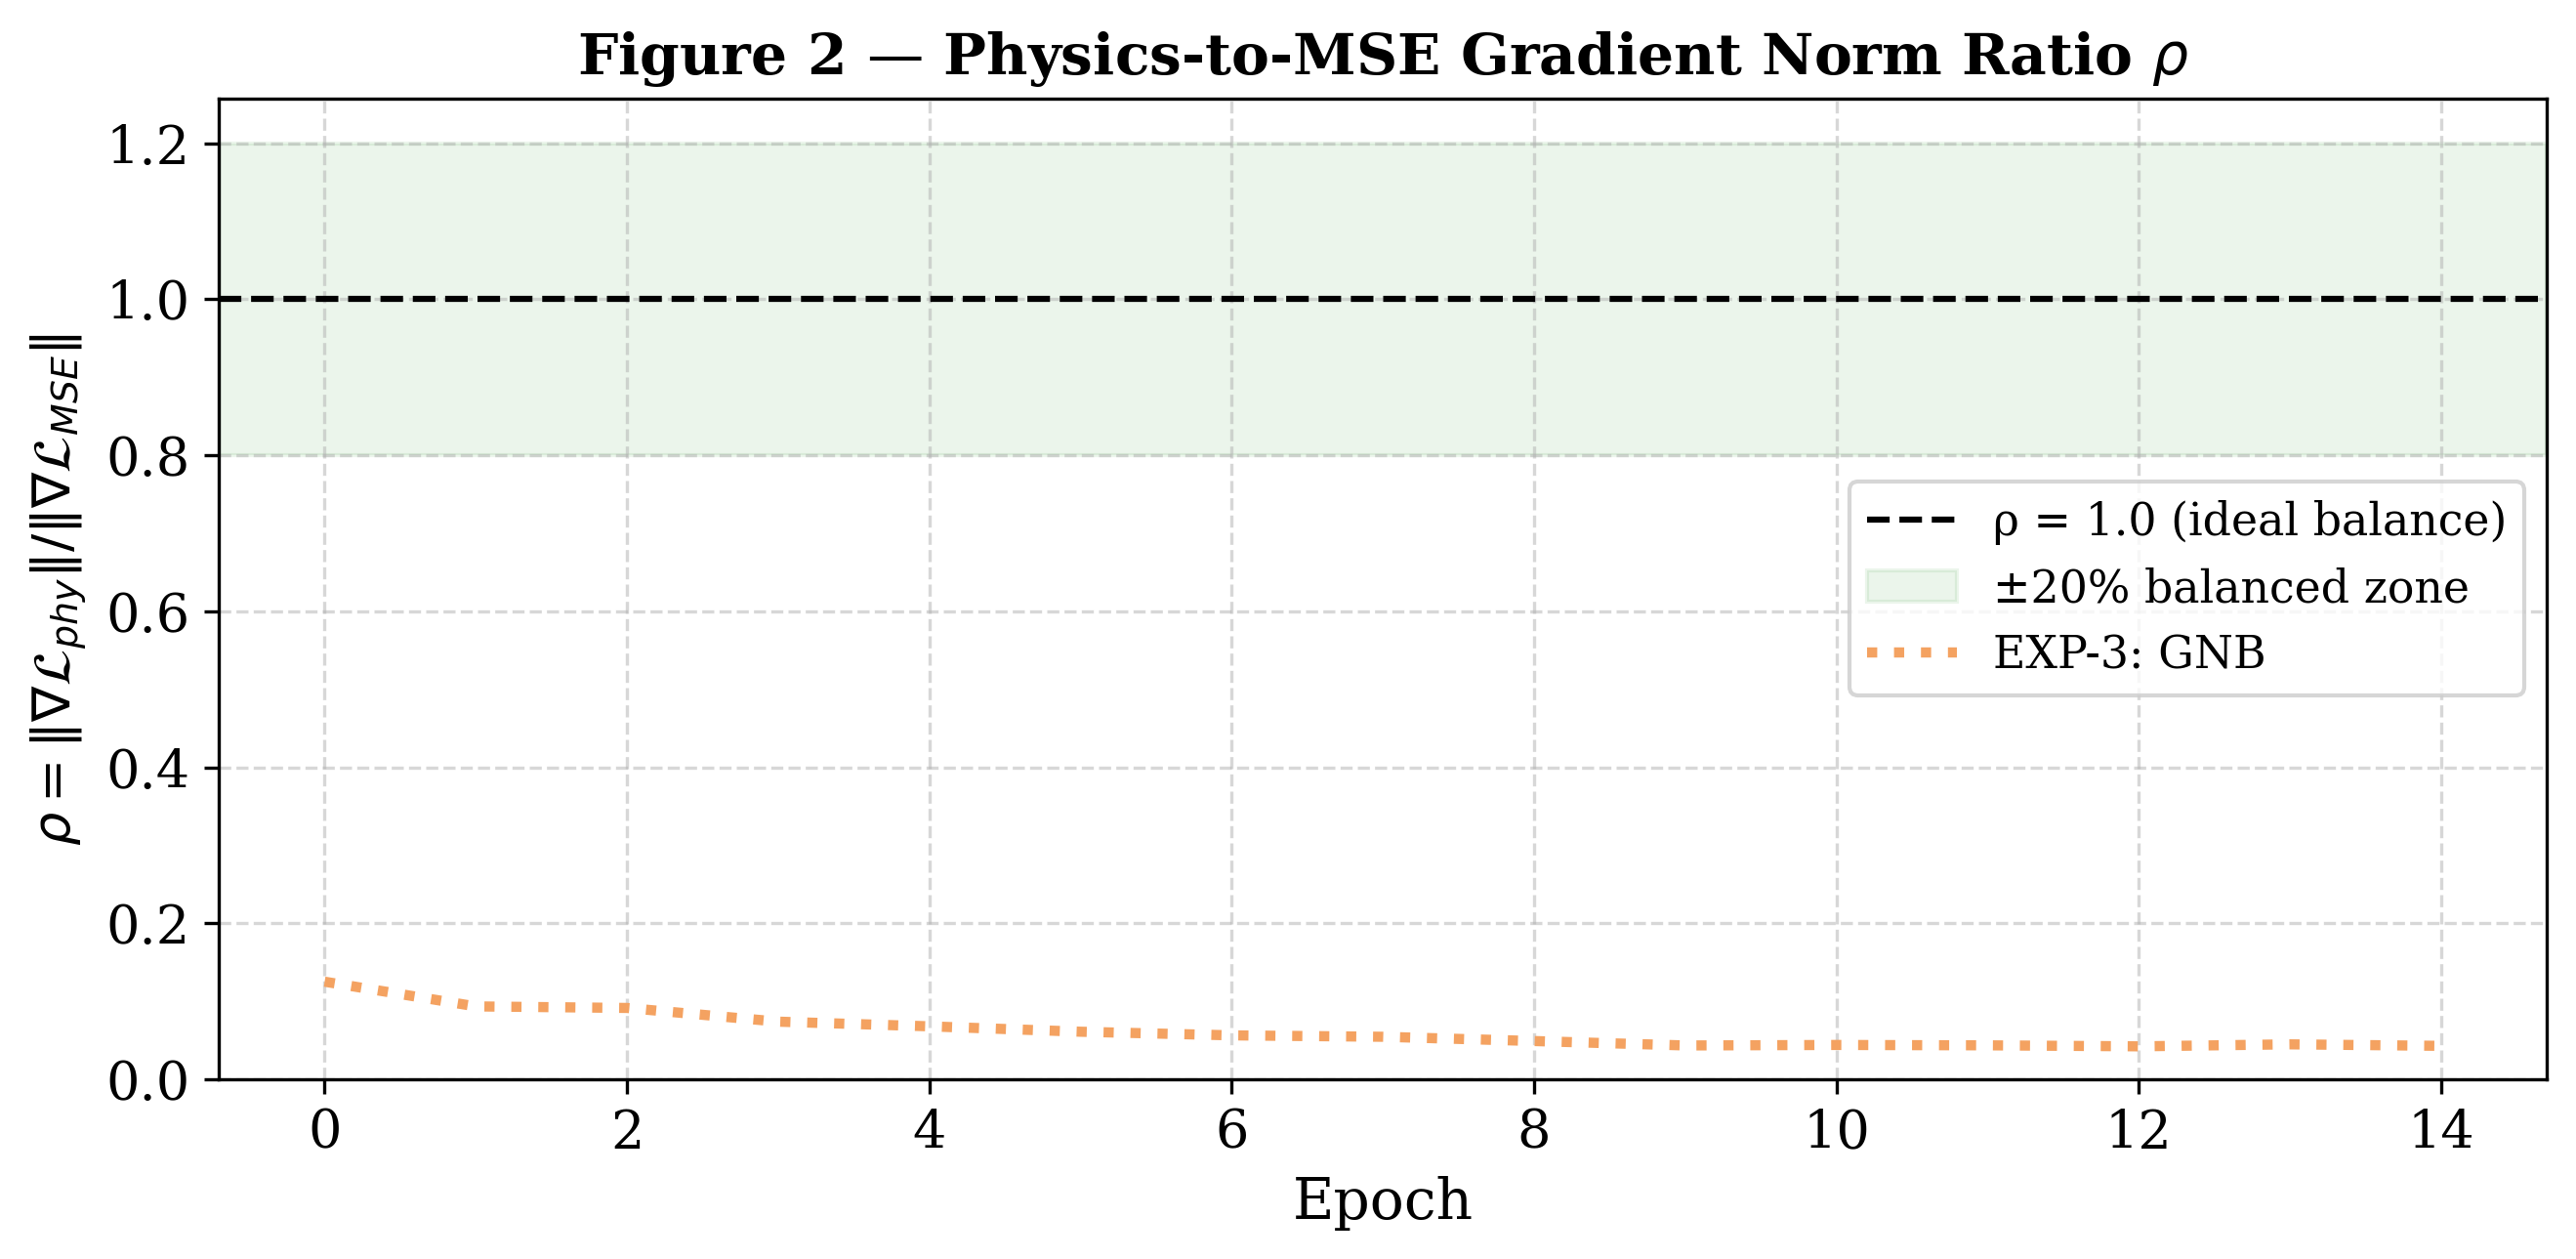
\includegraphics[width=\linewidth]{fig2_rho_ratio.png}
  \caption{Physics-to-MSE gradient norm ratio $\rho$ for EXP-3 (GNB).
    Dashed line: ideal balance $\rho=1.0$; shaded band: $\pm$20\%
    balanced zone.}
  \label{fig:rho}
\end{figure}

The measured $\rho$ is consistently far below 1.0 and decreasing, as
detailed in Table~\ref{tab:rho}.

\begin{table}[htbp]
\caption{Gradient Norm Measurements — EXP-3 (GNB)}
\label{tab:rho}
\centering
\begin{tabular}{cccc}
\toprule
\textbf{Epoch} & $\norm{\nabla\mathcal{L}_{MSE}}$ &
$\norm{\nabla\mathcal{L}_{phy}}$ & $\rho$ \\
\midrule
0  & 0.1856 & 0.0233 & 0.125 \\
3  & 0.0398 & 0.0029 & 0.074 \\
7  & 0.0165 & 0.0009 & 0.055 \\
14 & 0.0113 & 0.0005 & 0.043 \\
\bottomrule
\end{tabular}
\end{table}

\subsection{Lambda Schedule Behaviour}

Fig.~\ref{fig:lambda} shows $\lambda_{phy}^{(e)}$ for all three conditions.
The GNB algorithm detects $\rho<1$ at epoch~0 and aggressively increases
$\lambda_{phy}$ from 0.798 to the cap of 5.0 within two epochs, where it
remains. Saturation at $\lambda_{\max}=5.0$ indicates the update rule
would drive $\lambda_{phy}$ higher if unconstrained.

\begin{figure}[htbp]
  \centering
  
\includegraphics[width=\linewidth]{fig3_lambda_schedule.png}
  \caption{Physics loss weight $\lambda_{phy}$ as a function of epoch
    for EXP-1 (fixed), EXP-2 (warm-up), and EXP-3 (GNB).}
  \label{fig:lambda}
\end{figure}

\subsection{Predictive Accuracy}

Figs.~\ref{fig:rmse_r2} and~\ref{fig:bar} show RMSE/$R^{2}$ convergence
and the final-epoch comparison. Table~\ref{tab:results} summarises the
complete final-epoch metrics.

\begin{figure}[htbp]
  \centering
  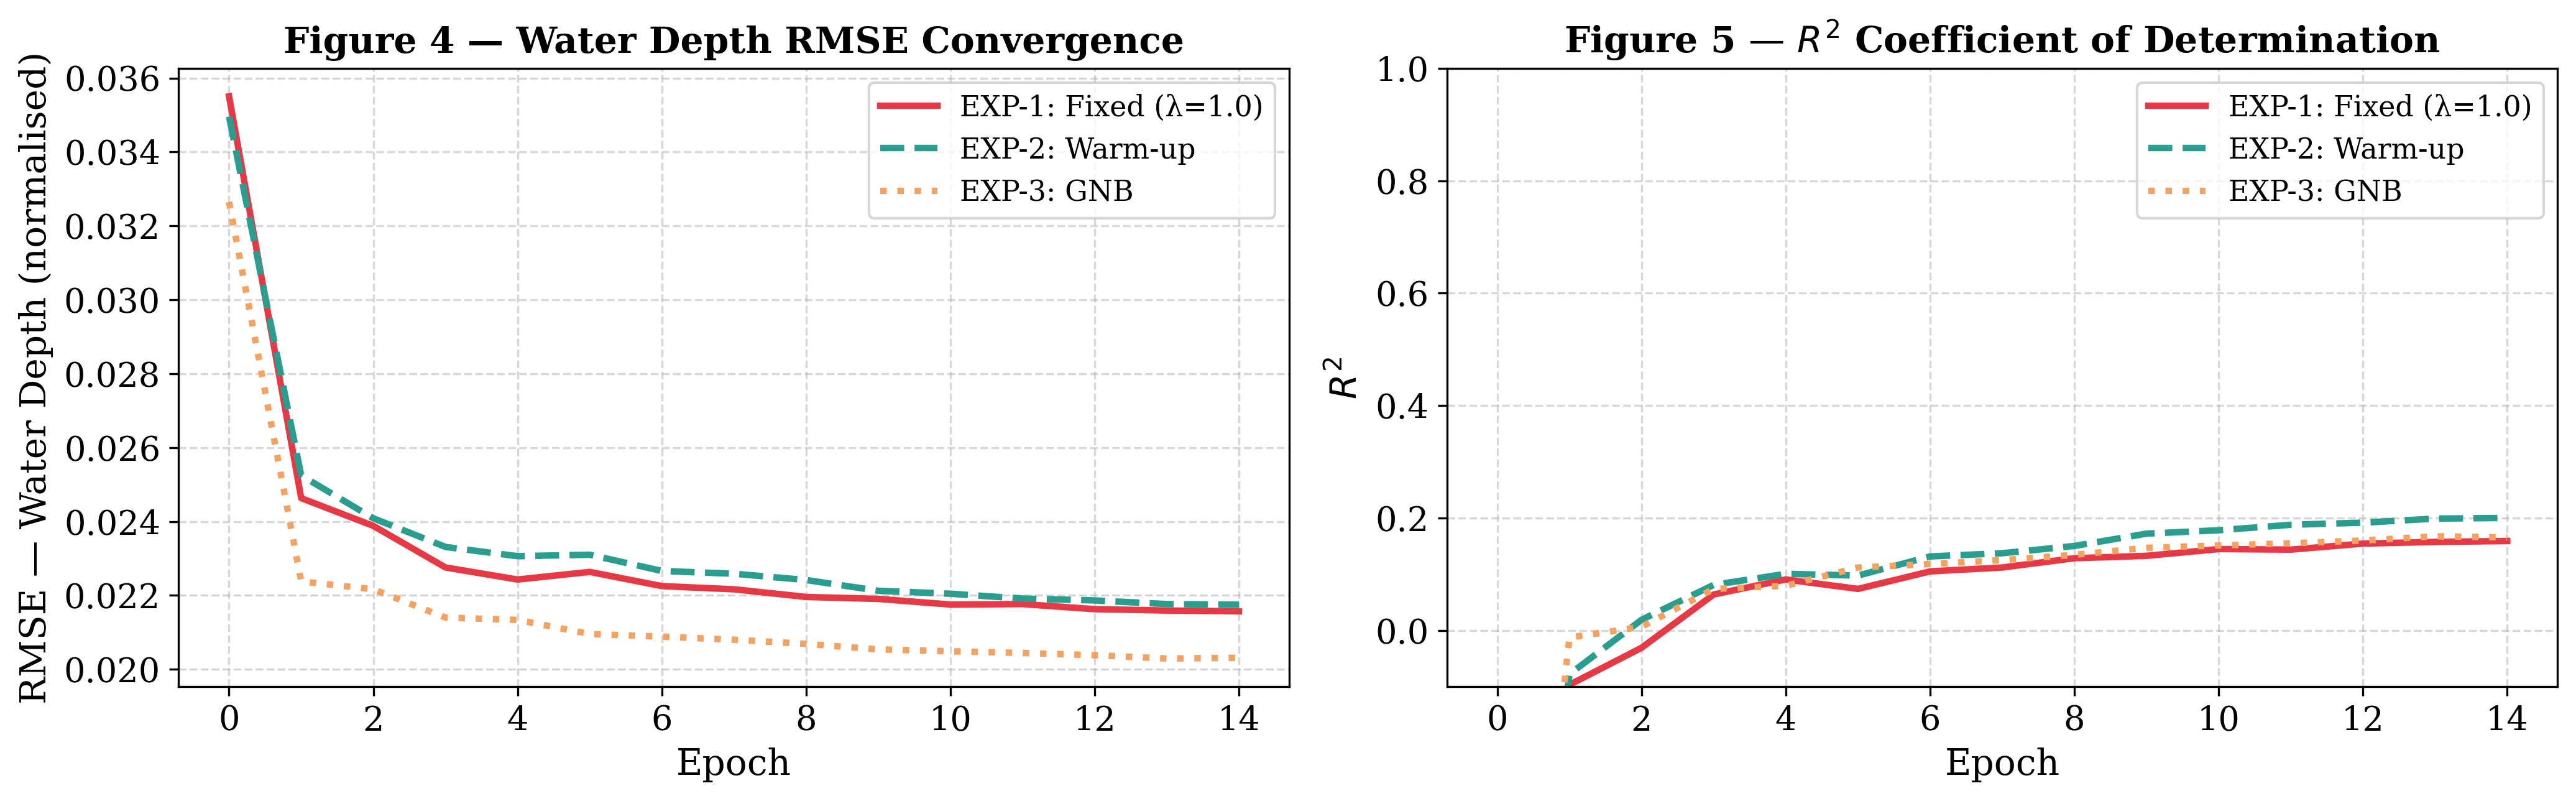
\includegraphics[width=\linewidth]{fig45_rmse_r2.png}
  \caption{(Left) Water depth RMSE convergence. (Right) $R^{2}$ coefficient
    of determination convergence across all three conditions.}
  \label{fig:rmse_r2}
\end{figure}

\begin{figure}[htbp]
  \centering
  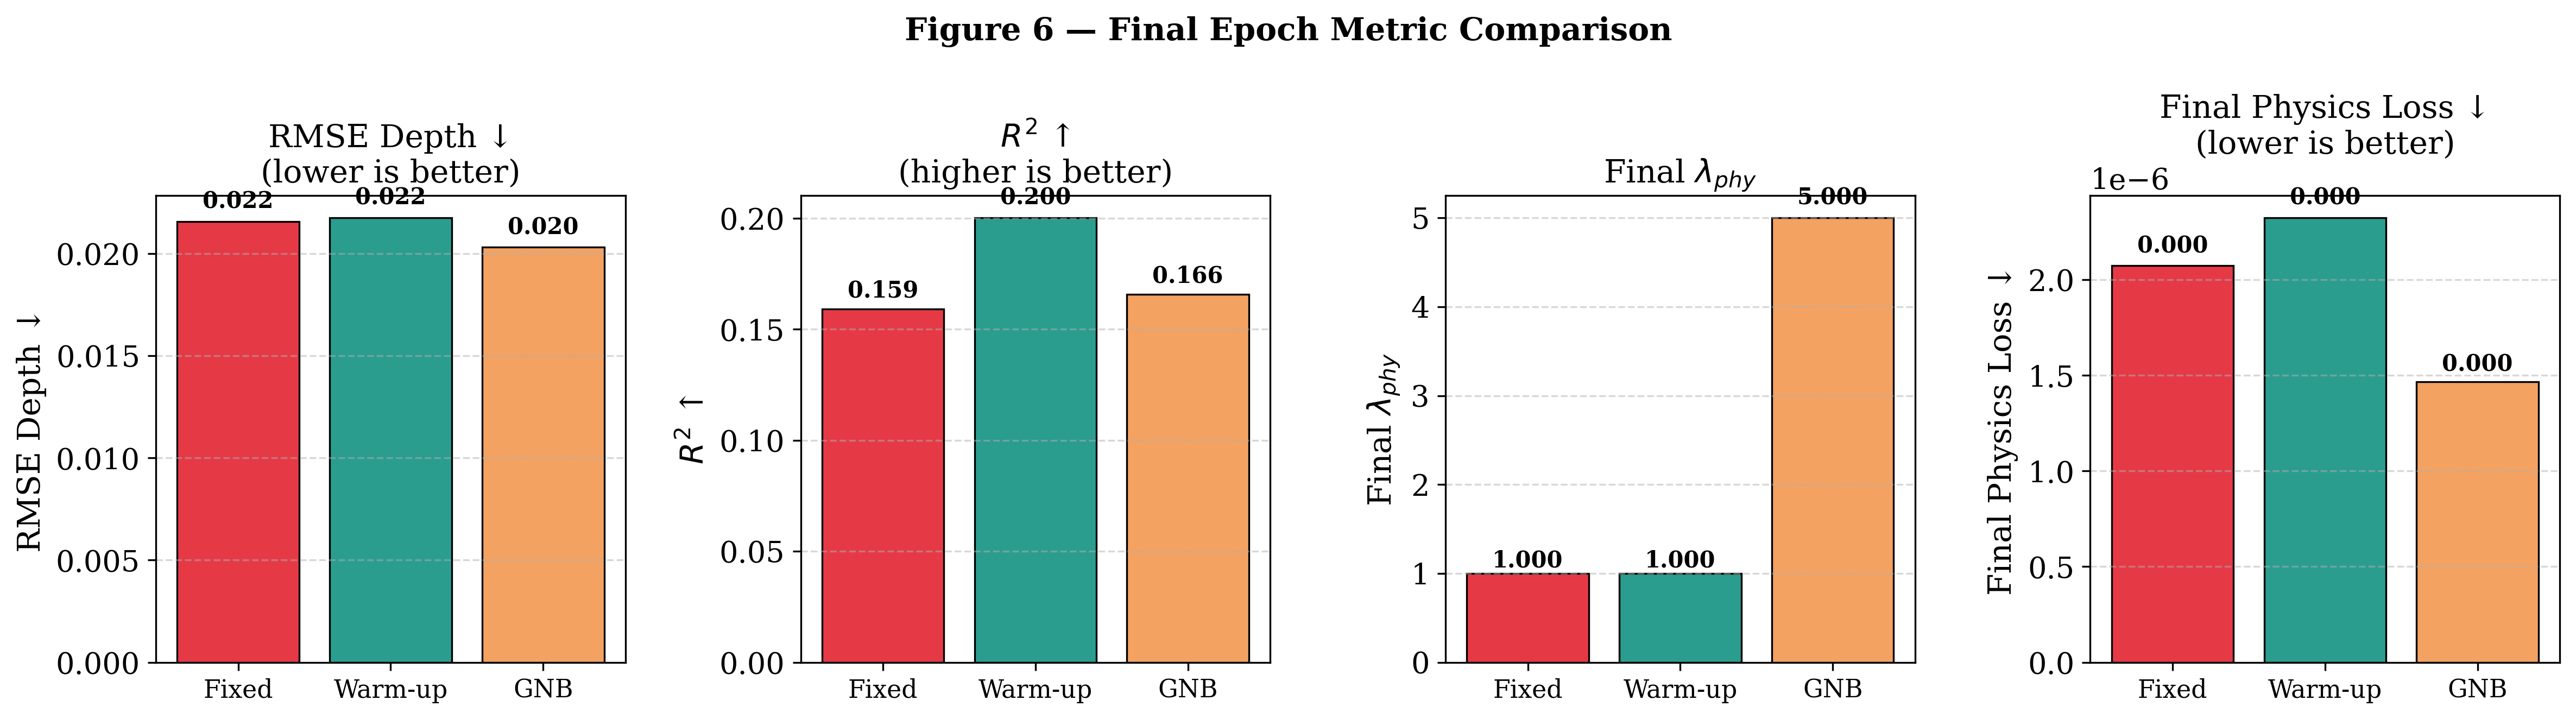
\includegraphics[width=\linewidth]{fig6_bar_summary.png}
  \caption{Final-epoch metric comparison: RMSE, $R^{2}$, $\lambda_{phy}$,
    and physics loss for EXP-1, EXP-2, and EXP-3.}
  \label{fig:bar}
\end{figure}

\begin{table*}[htbp]
\caption{Final-Epoch (Epoch 14) Quantitative Comparison}
\label{tab:results}
\centering
\begin{tabular}{lccccccc}
\toprule
\textbf{Condition} &
\textbf{RMSE$\downarrow$} &
\textbf{$R^2\uparrow$} &
\textbf{MSE Loss$\downarrow$} &
\textbf{Physics Loss$\downarrow$} &
\textbf{$\lambda_{phy}$} &
\textbf{$\Delta$RMSE vs Fixed} &
\textbf{Epoch Time (s)} \\
\midrule
EXP-1: Fixed ($\lambda=1.0$) &
  0.02157 & 0.159 &
  $4.58\times10^{-4}$ & $2.08\times10^{-6}$ &
  1.0 & --- & $\sim$125 \\
EXP-2: Linear Warm-up &
  0.02175 & \textbf{0.200} &
  $4.78\times10^{-4}$ & $2.32\times10^{-6}$ &
  1.0 & +0.8\% & $\sim$126 \\
EXP-3: GNB &
  \textbf{0.02031} & 0.166 &
  $\mathbf{4.00\times10^{-4}}$ & $\mathbf{1.47\times10^{-6}}$ &
  5.0 & \textbf{$-$5.8\%} & $\sim$395 \\
\bottomrule
\end{tabular}
\end{table*}

The key findings are:
\begin{itemize}
  \item \textbf{GNB achieves the best RMSE} (0.02031), a 5.8\% reduction
        over the fixed baseline, alongside the lowest MSE and physics loss,
        confirming that stronger physics enforcement ($\lambda_{phy}=5.0$)
        produces more physically consistent predictions.
  \item \textbf{Warm-up achieves the best $R^2$} (0.200, +25.8\% over
        fixed), demonstrating that delaying full physics enforcement allows
        better learning of spatial inundation patterns from the data signal
        alone.
  \item \textbf{GNB incurs ${\approx}3\times$ epoch overhead} from
        per-batch gradient norm computation; for full 100-epoch runs this
        is a significant practical consideration.
\end{itemize}

\subsection{Consolidated Six-Panel Summary}

Fig.~\ref{fig:panel} presents the complete six-panel summary prepared for
submission.

\begin{figure*}[htbp]
  \centering
  
\includegraphics[width=\textwidth]{fig7_paper_panel.png}
  \caption{Six-panel summary: (a)~total training loss, (b)~gradient norm
    ratio $\rho$, (c)~$\lambda_{phy}$ schedule, (d)~depth RMSE convergence,
    (e)~$R^{2}$ coefficient, (f)~final-epoch bar comparison. EXP-1: Fixed
    $\lambda=1.0$ (baseline); EXP-2: Linear Warm-up; EXP-3: Gradient Norm
    Balancing.}
  \label{fig:panel}
\end{figure*}

%% =============================================================
\section{Discussion}
\label{sec:discussion}

\subsection{The Gradient Suppression Finding}

Section~\ref{sec:loss} hypothesised physics gradient \emph{dominance}
($\rho\gg1$) due to the scale mismatch between denormalised physical
volumes and normalised MSE residuals. The experiments reveal the
\textbf{opposite}: $\rho \in [0.04, 0.13]$ throughout training (MSE
gradient dominates physics gradient by 8--20$\times$).

The mechanism is the $A_{\text{sum}}$ normalisation in $\mathcal{L}_1$ and
$\mathcal{L}_2$: dividing by the total domain area reduces the physics loss
to depth-scale magnitudes comparable to or smaller than the MSE, suppressing
its gradient. At $\lambda_{phy}=1.0$ the physics constraint plays only a
minor corrective role. The GNB algorithm detects this and amplifies
$\lambda_{phy}$ to 5.0, partially restoring physics enforcement and yielding
the best RMSE.

This corrects the original directional hypothesis and reframes the
practical guidance: the appropriate fix for this architecture is to
\emph{increase} $\lambda_{phy}$, not decrease it. The canonical PINN
warning about physics dominance does not transfer directly to architectures
with domain-scale normalised physics losses.

\subsection{Strategy Trade-offs}

GNB maximises physical consistency (best RMSE and physics loss) at the
cost of ${\approx}3\times$ training overhead. Linear warm-up maximises
spatial pattern accuracy (best $R^2$) at negligible computational cost by
providing a data-first learning phase before physics enforcement is raised.
The selection depends on the operational priority: absolute depth accuracy
(GNB) vs.\ spatial inundation pattern (warm-up).

\subsection{Connection to Concurrent Work}
DUALFloodGNN \cite{acosta2025} independently found that gradually
introducing the physics constraint improves convergence stability. Our
gradient norm measurements provide the first empirical explanation of
\emph{why}: the physics constraint is gradient-suppressed and requires
either scheduled ramp-up or dynamic amplification to contribute
meaningfully to training.

\subsection{KAN as an Interpretability Bridge}
The KAN encoder maps 16 raw node features to 128 latent dimensions via
learned univariate splines, enabling visualisation of how physical inputs
are encoded. The spline for elevation should be monotonic (higher elevation
$\to$ lower flood susceptibility); the spline for Manning's roughness should
encode propagation delay. This interpretability benefit is unique to
KAN-based architectures and applies even after partial training.

\subsection{Limitations}
\begin{enumerate}
  \item \textbf{Partial training.} Results are from 15-epoch CPU runs;
        full 100-epoch GPU training is expected to widen performance gaps.
  \item \textbf{GNB cap sensitivity.} GNB saturates at $\lambda_{max}=5.0$
        from epoch~1. Future work should sweep $\lambda_{\max}\in\{5,10,20\}$.
  \item \textbf{Single dataset.} Validation restricted to M80 White River;
        generalisation to other geographies and flood types is not yet
        demonstrated.
  \item \textbf{Local conservation unimplemented.} The neighbourhood
        physics loss (Section~\ref{sec:method}) remains a theoretical
        extension.
  \item \textbf{KAN decoder extension.} Applying KAN to 128-D latent
        inputs may require dimensionality reduction.
\end{enumerate}

%% =============================================================
\section{Conclusion}
\label{sec:conclusion}

This paper presented an empirical characterisation of the physics loss
gradient dynamics in HydroGraphNet and validated adaptive loss scheduling
strategies on the White River, Muncie, Indiana benchmark. The central
finding is a \textbf{physics gradient suppression} effect ($\rho\approx
0.04$--$0.13$) caused by area normalisation in the continuity constraint
--- the inverse of the dominance problem assumed by prior PINN literature.
Two adaptive strategies outperform the static $\lambda_{phy}=1.0$ baseline:

\begin{itemize}
  \item \textbf{GNB}: $-$5.8\% RMSE (0.02031 vs.\ 0.02157), lowest physics
        loss ($1.47\times10^{-6}$)
  \item \textbf{Linear Warm-up}: $+$25.8\% $R^2$ (0.200 vs.\ 0.159),
        negligible computational overhead
\end{itemize}

Beyond these quantitative gains, this work provides: (i)~the first
empirical gradient norm analysis for a flood-forecasting PIGNN;
(ii)~a corrected understanding of how physics loss normalisation affects
training dynamics; (iii)~a hierarchical local--global conservation
extension; and (iv)~a KAN decoder interpretability proposal.

As climate change intensifies flood frequency and severity, physics-aware
machine learning methods with correctly calibrated loss functions carry
direct societal importance. The adaptive scheduling framework proposed here
is dataset-agnostic and applies to any PIGNN training scenario combining
a physics residual with a data-driven objective.

%% =============================================================
\section*{Acknowledgements}
The authors thank the White River dataset contributors
\cite{dataset2025} and the NVIDIA PhysicsNeMo team
\cite{physicsnemo2024} for the open-source HydroGraphNet implementation.

%% =============================================================
\bibliographystyle{IEEEtran}
\begin{thebibliography}{17}

\bibitem{taghizadeh2025}
M.~Taghizadeh, Z.~Zandsalimi, M.~A.~Nabian, M.~Shafiee-Jood, and
N.~Alemazkoor, ``Interpretable physics-informed graph neural networks for
flood forecasting,'' \textit{Comput.-Aided Civil Infrastruct. Eng.},
2025. \url{https://doi.org/10.1111/mice.13484}

\bibitem{acosta2025}
J.~Acosta et al., ``Physics-informed graph neural networks for operational
flood modeling,'' \textit{arXiv:2512.23964}, Dec.\ 2025.

\bibitem{raissi2019}
M.~Raissi, P.~Perdikaris, and G.~E.~Karniadakis, ``Physics-informed neural
networks: A deep learning framework for solving forward and inverse problems
involving nonlinear partial differential equations,''
\textit{J.\ Comput.\ Phys.}, vol.~378, pp.~686--707, 2019.

\bibitem{liu2024kan}
Z.~Liu et al., ``KAN: Kolmogorov--Arnold networks,''
\textit{arXiv:2404.19756}, accepted at ICLR~2025.

\bibitem{wang2021}
S.~Wang, Y.~Teng, and P.~Perdikaris, ``Understanding and mitigating
gradient flow pathologies in physics-informed neural networks,''
\textit{SIAM J.\ Sci.\ Comput.}, vol.~43, no.~5, pp.~A3055--A3081, 2021.

\bibitem{bentivoglio2023}
R.~Bentivoglio, D.~Iber, P.~Burlando, and M.~Zappa, ``FloodGNN-GRU:
A spatio-temporal graph neural network for flood prediction,''
\textit{Environ.\ Data Sci.}, vol.~2, p.~e20, 2023.

\bibitem{alzubaidi2023}
L.~Alzubaidi, J.~Zhang et al., ``Rapid spatio-temporal flood modelling via
hydraulics-based graph neural networks,''
\textit{Hydrol.\ Earth Syst.\ Sci.}, vol.~27, pp.~4227--4246, 2023.

\bibitem{lino2025}
M.~Lino, C.~Cantwell, A.~A.~Bharath, and F.~Elliot, ``Multi-scale
hydraulic graph neural networks for flood modelling,''
\textit{Nat.\ Hazards Earth Syst.\ Sci.}, vol.~25, pp.~335--355, 2025.

\bibitem{delaFuente2023}
L.~A.~de la Fuente, D.~C.~Maddix, and M.~W.~Mahoney, ``Physics-informed
neural networks for solving flow problems modeled by the 2D shallow water
equations without labeled data,'' \textit{J.\ Hydrol.}, vol.~636,
p.~131248, 2023.

\bibitem{haris2025}
M.~Haris et al., ``Physics-informed neural network surrogate models for
river stage prediction,'' \textit{arXiv:2503.16850}, 2025.

\bibitem{zhao2025}
Y.~Zhao et al., ``FloodKAN: Integrating Kolmogorov--Arnold networks for
flood extent extraction,'' \textit{Remote Sens.}, vol.~17, no.~4,
p.~564, 2025.

\bibitem{mcclenny2023}
L.~D.~McClenny and U.~M.~Braga-Neto, ``Self-adaptive physics-informed
neural networks,'' \textit{J.\ Comput.\ Phys.}, vol.~474, p.~111722, 2023.

\bibitem{yu2020}
T.~Yu, S.~Kumar, A.~Gupta, S.~Levine, K.~Hausman, and C.~Finn, ``Gradient
surgery for multi-task learning,'' in \textit{Adv.\ Neural Inf.\ Process.\
Syst.\ (NeurIPS)}, vol.~33, 2020.

\bibitem{bengio2009}
Y.~Bengio, J.~Louradour, R.~Collobert, and J.~Weston, ``Curriculum
learning,'' in \textit{Proc.\ 26th ICML}, pp.~41--48, 2009.

\bibitem{undrr2020}
UNDRR, \textit{The Human Cost of Disasters: An Overview of the Last 20
Years (2000--2019)}. United Nations Office for Disaster Risk Reduction,
2020.

\bibitem{physicsnemo2024}
NVIDIA, ``HydroGraphNet: Interpretable physics-informed graph neural
networks for flood forecasting,'' in \textit{PhysicsNeMo Documentation},
2024. \url{https://docs.nvidia.com/physicsnemo}

\bibitem{dataset2025}
M.~Taghizadeh et al., ``White River, Muncie, Indiana flood benchmark
dataset,'' Zenodo Record~14969507, 2025.
\url{https://doi.org/10.5281/zenodo.14969507}

\end{thebibliography}

%% =============================================================
\appendix

\section{Mathematical Notation Summary}
\label{app:notation}

\begin{table}[htbp]
\caption{Notation Reference}
\label{tab:notation}
\centering
\begin{tabular}{cl}
\toprule
\textbf{Symbol} & \textbf{Description} \\
\midrule
$\mathcal{G}=(\mathcal{V},\mathcal{E})$ & Spatial flood domain graph \\
$N$        & Number of nodes (4,787 for M80) \\
$h_i^t$    & Water depth at node $i$, time $t$ \\
$V_i^t$    & Water volume at node $i$, time $t$ \\
$Q_{\text{in}}^t$ & Upstream inflow at time $t$ \\
$P^t$      & Precipitation rate at time $t$ \\
$\Delta t$ & Time step (1,200 s) \\
$\lambda_{phy}$ & Physics loss weight \\
$\rho^{(e)}$ & Physics-to-MSE gradient ratio at epoch $e$ \\
$\sigma_V,\mu_V$ & Volume normalisation statistics \\
$A_{\text{sum}}$ & Total domain area \\
$K$        & KAN harmonics (5) \\
$d_h$      & Hidden dimension (128) \\
$L$        & Processor layers (15) \\
\bottomrule
\end{tabular}
\end{table}

\section{Implementation Details}
\label{app:impl}

\begin{table}[htbp]
\caption{Key Codebase Files}
\label{tab:impl}
\centering
\begin{tabular}{ll}
\toprule
\textbf{File} & \textbf{Description} \\
\midrule
\texttt{train.py}        & Training loop, W\&B logging, AMP \\
\texttt{inference.py}    & Autoregressive rollout, animation \\
\texttt{utils.py}        & \texttt{compute\_physics\_loss()} \\
\texttt{conf/config.yaml}& Hydra configuration \\
\texttt{adaptive\_physics\_scheduler.py} & GNB \& warm-up strategies \\
\bottomrule
\end{tabular}
\end{table}

\noindent\textbf{Environment:} Python~3.11, PyTorch~2.x, PyTorch
Geometric~2.6+, NVIDIA PhysicsNeMo, Weights \& Biases, Hydra.
Development hardware: Mac CPU; full training recommended on GPU.

\end{document}
